% ----------------------------------------------------------------
\documentclass[12pt,a4paper]{article}

\usepackage[british,UKenglish]{babel}  %% Language
\usepackage[a4paper, margin=1in]{geometry} %% margins
\usepackage{natbib} %% References
\usepackage[a4paper,bookmarks=true, colorlinks=false]{hyperref} % Links - must be last package

\usepackage{graphicx}
\usepackage[section]{placeins}
\graphicspath{ {images/} }

\usepackage{tikz}
\usepackage{gantt}

\begin{document}

\title{Parallelize Operations on a Durable Queue by Using Log Structured Storage with Memory Interleaving}%
\author{Avinash D'Silva \\ 15028534 \\ MSc in Cloud Computing}%
\date{\today}
\maketitle

\begin{abstract}
In the recent years, Queues have become the de-facto standard for various purposes such as asynchronous processing, buffering and load balancing. Queues basically have two operations, enqueue and dequeue. These operations are parallel in theory but in practice when implemented as a durable queue, they tend to become more akin to an ACID compliant database system and hence loose their ability to perform operations in parallel. Durability of a queue cannot be compromised and yet at the same time, the need for performance is ever more increasing as queues have become the backbone of most distributed systems. This study will focus on Log Structured Storage along with Memory Interleaving and how a combination of these can make it possible for a queue to be durable as well as be able to perform parallel operations at the same time.
\end{abstract}

% TOC
\tableofcontents

\section{Introduction}

Queues are not a modern invention related to the field of Computer Science. They have existed well over the centuries. People queue up instinctively when there is a crowd for any given situation \citep{spieser2008stabilizing}. Queues particularly in the field of Computer science are known for their FIFO(First in First Out) data flow \citep{maclaren1969art}. Queues were initially used for simple well known tasks such as enqueueing a print task on a printer, for breadth first search and have applications in graph theory. \\

 The structure of a queue very simple to understand and implement and queues in the recent years have become the backbone of distributed systems \citep{lamport1978time}. They are used for asynchronous processing, message passing, buffering and load balancing \citep{lu2011join}. 

 The size of data that most public facing applications have to deal with has been growing. There is ever more data from different IoT devices, Cell phones and Communication satellites and hence this age is called the Age of Big Data \citep{10333611920150101} \citep{lohr2012age}.\\
 
 
 The distributed systems have come under heavy load due to this growth in the size of data. One of the important part of the distributed system, the queues are the most affected as these are the ones that carry and distribute the data throughout the system \citep{lamport1978time}. Queueing servers are becoming a bottleneck due to their fundamental shortcoming of not supporting parallel operations. The Figure \ref{fig:gull} shows how queues are implemented currently and shows how producers and consumers both use a single Write Ahead Log for durability. The Write Ahead Log only allows one operation at a time to be logged and hence queues aren't parallel due to this persistance layer.\\ 
 
 \begin{figure}
 	\centering
 	\textbf{}\par\medskip
 	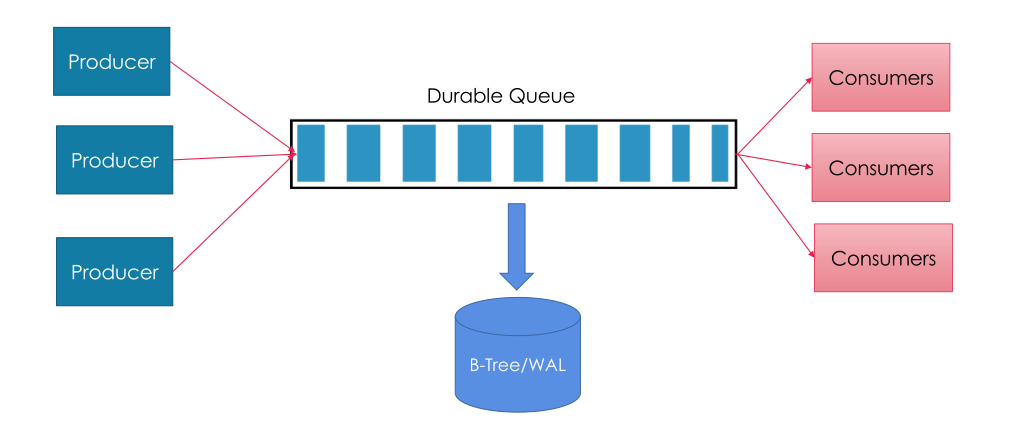
\includegraphics[scale=0.6]{1}
 	\caption{Overall architecture of the current queueing systems}
 	\label{fig:gull}
 \end{figure}
 
 

    
 Although queues are parallel in theory, they loose their parallel nature due to reliance on external disk based storage structures such as B-Trees and WAL(Write Ahead Log) for durability. Queueing servers use various workarounds such as fan out queues and clustering as shown in Figure \ref{fig:gdulld} \citep{albrecht2013making}.\\
 
 
\begin{figure}
   	\centering
   	\textbf{}\par\medskip
   	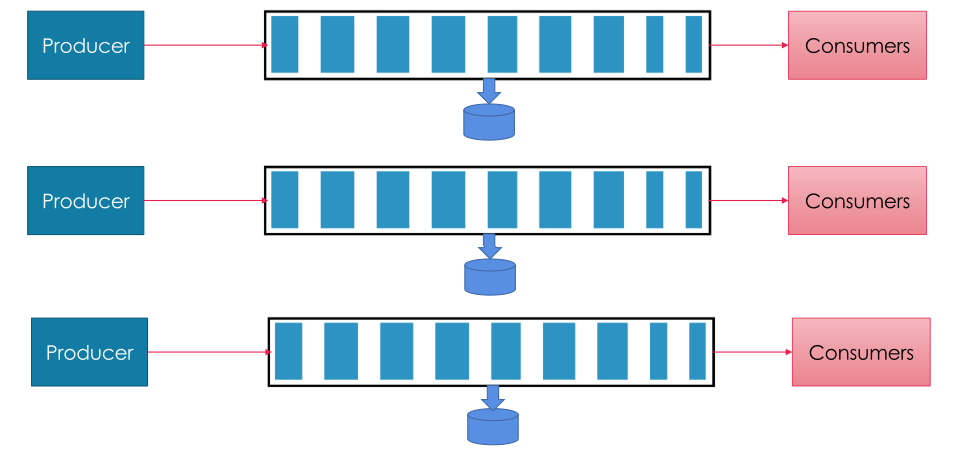
\includegraphics[scale=0.6]{2}
   	\caption{Achitecture of a clustered queueing systems}
   	\label{fig:gdulld}
\end{figure}
     
 
 The method of fanning out or clustering involves using multiple queues instead of a single queue to better handle the load. These multiple queues are abstracted as a single queue. One queueing server acts as a master while the rest act as slaves. These queues can be either mirror replicated or sharded \citep{albrecht2013making}. This type of setup is widely used in the industry today and almost all major queuing servers support the feature of clustering \citep{kermarrec2013xl}. But this doesn't solve the fundamental problem of durable queues not being parallel. This proposal describes the ways and means to parallelize operations on a durable queue using a combination of well known technique of memory interleaving and Log Structured Storage.
 

 
\section{Literature Review}
\label{ric:litreview} % use labels to point to parts of your work

 Various file formats have been defined, one of the oldest and the most widely used is the distributed systems have come under heavy load due to this growth in the size of data. One of the important part of the distributed system, the queues are the most affected as these are the ones that carry and distribute the data throughout the system \citep{lamport1978time}. Queueing servers are becoming a bottleneck due to their fundamental shortcoming of not supporting parallel operations. Queueing servers use various workarounds such as fan out queues and clustering \citep{albrecht2013making}.
 
 The method of fanning out or clustering involves using multiple queues instead of a single queue to better handle the load. These multiple queues are abstracted as a single queue. One queueing server acts as a master while the rest act as slaves. These queues can be either mirror replicated or sharded \citep{albrecht2013making}.

\section{Research Method and Specification}

 The distributed systems have come under heavy load due to this growth in the size of data. One of the important part of the distributed system, the queues are the most affected as these are the ones that carry and distribute the data throughout the system \citep{lamport1978time}. Queueing servers are becoming a bottleneck due to their fundamental shortcoming of not supporting parallel operations. Queueing servers use various workarounds such as fan out queues and clustering \citep{albrecht2013making}.
 
 \subsection{Gantt Chart}
 
 The following gantt chart shows the number of weeks on the X-Axis and the tasks that are to be the executed on the Y-Axis.
 
 \begin{gantt}{11}{12}
 \begin{ganttitle}
 \numtitle{1}{1}{12}{1}
 \end{ganttitle}
 \ganttbar{Install Queue}{0}{0.5}
 \ganttbar{Bench. Server}{0.5}{0.5}
 \ganttbar{Develop Layer}{1}{2}
 \ganttbar{Replace Layer}{3}{1}
 \ganttbar{Re-Run Benchs.}{4}{0.5}
 \ganttbar{Compare Benchs.}{4.5}{1.5}
 \ganttbar{Bench. on VM}{6}{2}
 \ganttbar{failure simulation}{8}{2}
 \ganttbar{Compile results}{10}{1}
 \ganttbar{Finalize paper}{11}{1}
 \end{gantt}

 \bigskip
 The first phase involves installing and configuring an open source queueing server. After the installation, several benchmarks are run to see how the server performs in different conditions. The conditions will include different processor speeds, different number of processor cores and varying size of memory. Then the proposed solution is developed and this solution will replace the previously benchmarked queueing servers' storage layer. After the replacement, The benchmark tests are performed again and then compared. Then both the versions are compared based on how they perform on a virtualized environment. To test the effectiveness of memory interleaving, hardware failure is simualated. These tests along with the benchmarks results are  compiled and the paper is finalized based on these results.
 

% references
\bibliographystyle{dcu}
\bibliography{mmur}

\end{document}